\chapter{Введение в математику}
\section{Введение в математическую логику}
\subsection{Логические символы}

%\begin{table}[H]
  \centering
  \begin{tabular}{ |l|l|l| }
    \hline
    \textbf{Символ} & \textbf{Название} & \textbf{Значение} \\ 
    \hline
    \hline
    $\forall$ (англ. all --- все) & Квантор общности & Для любого, для всякого \\  
    \hline
    $\exists$ (англ. exists --- существует) & Квантор существования & Существует \\  
    \hline
    $\nexists$ &  & Не существует \\
    \hline
    $\exists$! &  & Существует единственный \\
    \hline
    $\neg P(x)$, $\overline{P(x)}$ & Знак отрицания & Не $P(x)$ \\
    \hline
    $\wedge$ & Конъюнкция & Логическое "И" \\
    \hline
    $\vee$ & Дизъюнкция & Логическое "ИЛИ" \\
    \hline
    $\Rightarrow$ & Следование, импликация & A влечет B, из A следует B  \\
    \hline
    $\Leftrightarrow$ & Эквивалентность, равносильность & A эквивалентно  B\\
    \hline
  \end{tabular}
  \caption{Логические символы}
  \label{table:quantors_explained}
\end{table}


\begin{table}[H]
  \centering
  \begin{tabular}{ |l|l|l| }
    \hline
    \textbf{Символ} & \textbf{Название} & \textbf{Значение} \\ 
    \hline
    \hline
    $\forall$ (англ. all --- все) & Квантор общности & Для любого, для всякого \\  
    \hline
    $\exists$ (англ. exists --- существует) & Квантор существования & Существует \\  
    \hline
    $\nexists$ &  & Не существует \\
    \hline
    $\exists$! &  & Существует единственный \\
    \hline
    $\neg P(x)$, $\overline{P(x)}$ & Знак отрицания & Не $P(x)$ \\
    \hline
    $\wedge$ & Конъюнкция & Логическое "И" \\
    \hline
    $\vee$ & Дизъюнкция & Логическое "ИЛИ" \\
    \hline
    $\Rightarrow$ & Следование, импликация & A влечет B, из A следует B  \\
    \hline
    $\Leftrightarrow$ & Эквивалентность, равносильность & A эквивалентно  B\\
    \hline
  \end{tabular}
  \caption{Логические символы}
  \label{table:quantors_explained}
\end{table}



\dfn{Высказывание}{\textbf{Высказыванием}
  называется любое повествовательное предложение, которому можно придать значение истинности, т. е. сказать истинно оно или ложно.
}

\dfn{Предикат}{\textbf{Одноместным предикатом}
  называется высказывание, зависящее от некоторого аргумента, принадлежащего к некоторому множеству $X$.
}

\nt{
  \begin{itemize}
     \item $\forall x \in X: P(x)$ --- для любого $x$ из множества $X$ выполнено $P(x)$
     \item $\exists x \in X: P(x)$ --- существует такое $x$ из множества $X$ выполнено $P(x)$
  \end{itemize}
}

\nt{
  Из определения квантора общности и квантора существования следуют правила отрицания кванторов:
    $$\overline{\forall x \in X: P(x)} \Leftrightarrow \exists x \in X: \overline{P(x)} $$
    $$\overline{\exists x \in X: P(x)} \Leftrightarrow \forall x \in X: \overline{P(x)} $$
  Т.е. для того, чтобы найти отрицание некоторого предиката, необходимо все $\forall$ заменить на $\exists$, а $\exists$ заменить на $\forall$.
}

\nt{
  В кванторной записти одноименные кванторы, идущие подряд, можно менять местами. Разные кванторы менять местами \textbf{нельзя}!
}



\subsection{Теоремы}

\dfn{Теорема}{\textbf{Теоремой}
  называется утверждение, истинность которого устанавливается посредством доказательства.
}

В математике теоремы имеют вид импликации:
$$P \Rightarrow Q$$

С теоремой $P \Rightarrow Q$ связаны следующие утверждения:
\begin{enumerate}
  \item $Q \Rightarrow P$ --- обратная теорема
  \item $\overline{P} \Rightarrow \overline{Q}$ --- противоположная теорема
  \item $\overline{Q} \Rightarrow \overline{P}$ --- теорема, противоположная обратной
\end{enumerate}

\dfn{Критерий}{
  Если $P \Rightarrow Q \wedge Q \Rightarrow P$ истинно, то утверждения $P$ и $Q$ эквивалентны ($P \Leftrightarrow Q$) и называются \textbf{критерием}. Иначе говорят, что $P$ необходимо и достаточно для $Q$ или $P$ есть характеристическое свойство для $Q$
}

\nt{
  Иногда критерий может носить более сложный характер. Например, утверждается, что некоторые утверждения $P_1, P_2, \ldots, P_n$ эквивалентны. Такой критерий удобно доказывать с помощью круговой схемы:

  $$P_1 \Rightarrow P_2 \Rightarrow \ldots \Rightarrow P_n \Rightarrow P_1$$
}



\section{Основы теории множеств}
\subsection{Множество и способы его задания}

\dfn{Множество}{\textbf{Множество}
  есть первичное, неопределимое понятие математики.
}

\nt{
  Под множеством мы понимаем некоторую совокумность объектов произвольной природы, объединенных каким-либо свойством. Создателем теории множеств является Георг Кантор, ему принадлежит следующая фраза: "Множество есть многое, мыслимое нами как единое".
}

Элементы множества обозначаются строчными латинскими буквами: $a$, $b$, $c$, ... .
Сами множества обозначаются заглавными латинскими буквами: $A$, $B$, $C$, ... .

Задать множество --- значит определить, какие объекты \textbf{принадлежат множеству $a \in A$}, а какие \textbf{не принадлежат множеству $a \notin A$.}

\dfn{Пустое множество}{\textbf{Пустым множеством}
  $\varnothing$ называется множество, не содержащее элементов.
}


\textbf{Способы задания множества:}
\begin{enumerate}[label=\bfseries\tiny\protect\circled{\small\arabic*}]
  \item \label{n:1} \textbf{\textit{Перечисление}}, например:
    $$X = \{a, b, c\}$$
    Множество $X$ состоит из элементов $a, b, c$. Данный метод чаще всего используется для задания конечных множеств.
  \item \label{n:2} \textbf{\textit{Индексация}} --- перечисление, при котором индексы задаются посредством некоторого другого множества:
    $$X = \{x_\alpha \}_{\alpha \in I},$$ где $I$ --- множетсво  индексов.
  \item \label{n:3} \textbf{\textit{С помощью характеристического свойства}}.
    Используется, когда имеется некоторое свойство, которым обладают элементы данного множества и которым одновременно не обладают все прочие элементы.
    \ex{}{
      Например, точки на окружности единичного радиуса можно задать следующим образом:
      $$X = \{ (x,y) : x^2 + y^2 = 1, x, y \in \bbR\}$$
    }
\end{enumerate}



\subsection{Вложение и равенство множеств}

\dfn{Подмножество}{
  Множество $A$ называется \textbf{подмножеством множества $B$}, если любой элемент из $A$ принадлежит $B$:

  $$A \subset B \xLeftrightarrow{\text{def}} \forall a \in A : a \in B $$
}

\dfn{Ревенство множеств}{
  Множества $A$ и $B$ называются \textbf{равными}, если $A$ является подмножеством $B$ и $B$ является подмножеством $A$:

  $$A = B \xLeftrightarrow{\text{def}} (A \subset B) \wedge (B \subset A)$$
}

\nt{$A \subset B$ не исключает $A = B$.}

\dfn{Собственное подмножество}{
  Если ($A \subset B) \wedge (A \neq B)$, то $A$ называется \textbf{собвственным подмножеством $B$}. Иначе,

  $$ A - \text{собственное подмножество} \xLeftrightarrow{\text{def}} (\forall a \in A: a \in B) \wedge (\exists b \in B : b \notin A) $$
}



\subsection{Операции над множествами}

\dfn{Объединение множеств}{
  \textbf{Объединением множеств $A$ и $B$}  называется множество $A \cup B$, состоящее их элементов, принадлежащих хотя бы одному из множеств $A$ и $B$:
  $$A \cup B = \{x: (x \in A) \vee (x \in B) \}$$
  \def\leftcircle{(-1,0) circle (2 cm)}
\def\rightcircle{(1,0) circle (2 cm)}
\begin{figure}[H]
  \centering
  \label{tikzpic:set_union}
  \begin{tikzpicture}
    \fill[red!30] \rightcircle;
    \fill[red!30] \leftcircle;

    \draw \leftcircle;
    \draw \rightcircle;
    \draw (-3,1.6) node {$A$};
    \draw (3,1.6) node {$B$};
    \draw (-5,0) node {$A \cup B = $};
    \draw (5,0) node {\text{     }};
  \end{tikzpicture}
  \caption{Объединение множеств}
\end{figure}


}

\dfn{Пересечение множеств}{\textbf{Пересечением множеств $A$ и $B$}
  называется множество $A \cap B$, состоящее их элементов, принадлежащих одновременно к обоим мноежством $A$ и $B$:
  $$A \cap B = \{x: (x \in A) \wedge (x \in B) \}$$
  \def\leftcircle{(-1,0) circle (2 cm)}
\def\rightcircle{(1,0) circle (2 cm)}

\begin{figure}[H]
  \centering
  \label{tikzpic:set_intersection}
  \begin{tikzpicture}
    \begin{scope}
      \clip \leftcircle;
      \fill[red!30] \rightcircle;
    \end{scope}
            
    \draw \leftcircle;
    \draw \rightcircle;
    \draw (-3,1.6) node {$A$};
    \draw (3,1.6) node {$B$};
    \draw (-5,0) node {$A \cap B = $};
    \draw (5,0) node {\text{     }};
  \end{tikzpicture}
  \caption{Пересечение множеств}
\end{figure}


}

\nt{
  Объединение совокупности множеств обозначается следующим образом:
  $$\underset{\alpha \in I}{\cup}A_{\alpha} \text{ или } \underset{\alpha}{\cup}A_{\alpha}$$

  Пересечение совокупности множеств обозначается так:
  $$\underset{\alpha \in I}{\cap}A_{\alpha} \text{ или } \underset{\alpha}{\cap}A_{\alpha}$$
}

\dfn{Разность множеств}{\textbf{Разностью множеств}
  $A$ и $B$ называется множество $A \setminus B$, состоящее из элементов, принадлежащих $A$, но непринадлижащих $B$:
  $$A \setminus B \xLeftrightarrow{\text{def}} \{x: (x \in A)\wedge (x\notin B) \}$$

  \def\leftcircle{(-1,0) circle (2 cm)}
\def\rightcircle{(1,0) circle (2 cm)}

\begin{figure}[H]
  \centering
  \label{tikzpic:set_minus}
  \begin{tikzpicture}
    \begin{scope}
      \clip \rightcircle (-3,-2) rectangle (3,2);;
      \fill[red!30] \leftcircle;
    \end{scope}
    
      \draw \leftcircle;
      \draw \rightcircle;
      \draw (-3,1.6) node {$A$};
      \draw (3,1.6) node {$B$};
      \draw (-5,0) node {$A \setminus B = $};
      \draw (5,0) node {\text{     }};
  \end{tikzpicture}
  \caption{Разность множеств}
\end{figure}


}

\dfn{Симметричная разность множеств}{\textbf{Симметричной разностью множеств}
  $A$ и $B$ называется множество $A \triangle B$, состоящее из элементов, принадлежащих объединению этих множеств, но непринадлижащих их пересечению:
  $$A \triangle B \xLeftrightarrow{\text{def}} (A \cup B)\setminus (A \cap B) \}$$

  \def\leftcircle{(-1,0) circle (2 cm)}
\def\rightcircle{(1,0) circle (2 cm)}
\begin{figure}[H]
  \centering
  \label{tikzpic:set_sym_minus}
   \begin{tikzpicture}
    \begin{scope}
      \clip \rightcircle (-3,-2) rectangle (3,2);;
      \fill[red!30] \leftcircle;
    \end{scope}
    \begin{scope}
      \clip \leftcircle (-3,-2) rectangle (3,2);;
      \fill[red!30] \rightcircle;
    \end{scope}
            
    \draw \leftcircle;
    \draw \rightcircle;
    \draw (-3,1.6) node {$A$};
    \draw (3,1.6) node {$B$};
    \draw (-5,0) node {$A \triangle B = $};
    \draw (5,0) node {\text{     }};
  \end{tikzpicture} 
  \caption{Симметричная разность}
\end{figure}


}

\dfn{Дополнение до множества}{
  Пусть $A \subset B$. \textbf{Дополнением множества} $A$ до множества $B$ называется множество:
  $$A^{C}_{B} \xLeftrightarrow{\text{def}} \{x: (x \in B)\wedge (x\notin A) \}$$
  \begin{figure}[H]
  \centering
  \label{tikzpic:set_complement}
  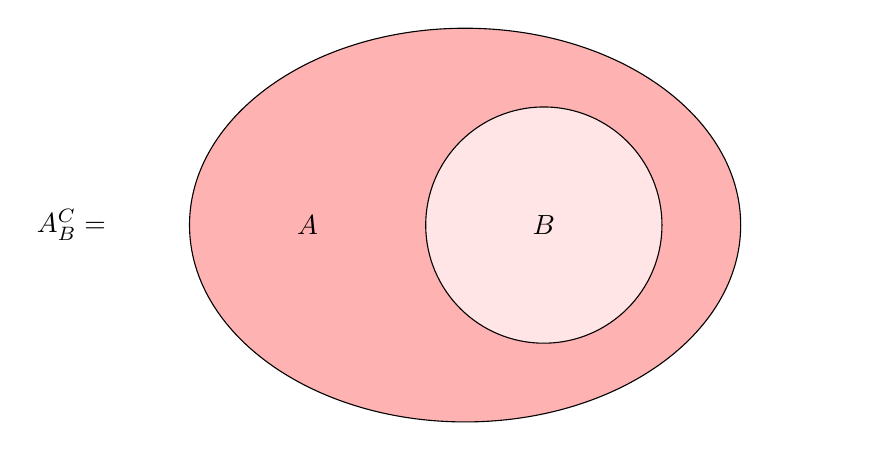
\begin{tikzpicture}
	  \fill[red!30] (0,0) ellipse (3.5 cm and 2.5 cm);
	  \fill[red!10] (1,0) circle (1.5 cm);

    \draw (0,0) ellipse (3.5 cm and 2.5 cm);
    \draw (1,0) circle (1.5 cm);
    \draw (-2,0) node {$A$};
    \draw (1,0) node {$B$};
    \draw (-5,0) node {$A^{C}_{B} = $};
    \draw (5,0) node {\text{     }};
  \end{tikzpicture}
  \caption{Дополнение до множестваh}
\end{figure}


}



\subsection{Свойства операций над множествами}

\begin{enumerate}[label=\bfseries\tiny\protect\circled{\small\arabic*}]
		\item \label{n:1} $A \cup B = B \cup A$ --- коммутативность объединения
		\item \label{n:2} $A \cap B = B \cap A$ --- коммутативность пересечения
		\item \label{n:3} $(A \cup B) \cup C = A \cup (B \cup C)$ --- ассоциативность объединения
		\item \label{n:4} $(A \cap B) \cap C = A \cap (B \cap C)$ --- ассоциативность пересечения
		\item \label{n:5} $A \cup (B \cap C) = (A \cup B) \cap (A \cup C)$ --- дистрибутивность объединения относительно пересечения
		\item \label{n:6} $A \cap (B \cup C) = (A \cap B) \cup (A \cap C)$ --- дистрибутивность пересечения относительно объединения
		\item \label{n:7} $(A \cup B)^{C} = A^{C} \cap B^{C} $ --- закон Де Моргана
		\item \label{n:8} $(A \cap B)^{C} = A^{C} \cup B^{C} $ --- закон Де Моргана
		\item \label{n:7} $(A^{C})^{C}$ --- закон дополнения
\end{enumerate}

\nt{Для доказательства свойств операций над множествами необходимо показать, что элемент, принадлежащий левой части равенства, принадлежит правой его части и наоборот.}



\section{Введение в математический анализ}
\subsection{Метод математической индукции}

\clm{Метод матиндукции}{}{
	Пусть $P(n)$ --- некоторое утверждение, зависящее от натурального аргумента $n 		\in \bbN$ (гипотеза). $P(n)$ можно доказать \textbf{методом математической 				индукции}. Если $P(1)$ верно (\textbf{база индукции}) и из верности $P(k)$ 				следует верность $P(k+1)$ ($P(k) \Rightarrow P(k+1)$ --- \textbf{индуктивный 			переход}), то $P(n)$ верно для любого натурального аргумента ($\forall n \in 			\bbN : P(n)$).
}

\nt{База индукции может быть любым $k_0 \in \bbN$. Тогда $P(n)$ будет выполняться $\forall n \geq k_0 $.}

\ex{Неравенство Бернулли}{
  $$(1+h)^n \geq 1 + nh, \text{  } (n > -1 , \text{  } n \in \bbN \cup \{0\})$$
  \begin{enumerate}
		\item \textbf{База индукции:} $n = 0: 1 \geq 1 \Rightarrow \text{истина} $
		\item \textbf{Индуктивное предположение:} предположим, что $(1+h)^k \geq 1 + kh$ истинно.
		\item \textbf{Индуктивный переход:}
		$$(1+h)^k \geq 1 + kh \text{  } |\cdot (1+h)$$
		$$(1+h)^{k+1} \geq 1 + kh + h + kh^2 \geq 1 + (1+k)h$$
		$$(1+h)^{k+1} \geq 1 + (1+k)h$$
		Согласно методу математической индукции неравенство Бернулли верно $\forall n \in \bbN \cup \{0\}$.
  \end{enumerate}
}

\subsection{Бином Ньютона}
\dfn{Сочетания}{
  Пусть $A = \{ a_1, a_2, ..., a_3\} $. \textbf{Сочетанием} из $n$  по $k$ называется любой набор $k$ элементов из заданного набора A. \textbf{Количество сочетаний} из $n$ по $k$ равно:
  $$C^k_n = \binom{n}{k} = \frac{n!}{k!(n-k)!} \text{, где } n! = 1 \cdot 2 \cdot 3 \cdot ... \cdot n, \text{ } 0! = 1$$
}

\textbf{Свойства сочетаний:}
\begin{enumerate}[label=\bfseries\tiny\protect\circled{\small\arabic*}]
	\item $C^0_n = C^n_n = 1$
  \item $C^k_n = C^{n-k}_n$
	\item $C^k_n + C^{k-1}_n = C^{k}_{n+1}$, доказательство:
  	$$C^k_n + C^{k-1}_n = \frac{n!}{k!(n-k)!} + \frac{n!}{(k-1)!(n-k+1)!} = 
  	\frac{n!(n-k+1 + k)}{k!(n-k+1)} = \frac{(n+1)!}{k!((n+1)-k)} = C^{k}_{n+1}$$
\end{enumerate}

\thm{Бином Ньютона}{
	$$(a+b)^n = C^0_n a^n b^0 + C^1_n a^{n-1} b^1 + ... + C^n_n a^0 b^n =
	\sum_{k=0}^{n} C^k_n a^{n-k} b^{k} $$
	$$\forall n \in \bbN, \forall a, b \in \bbR $$

	\textbf{Доказательство:}
	\begin{enumerate}
		\item База индукции: для $n=1 \Rightarrow (a+b)^1 = C^0_1 a^1 b^0 + C^1_1 a^0 b^1 = a + b$
		\item Пусть $(a+b)^m = \sum_{k=0}^{m} C^k_m a^{m-k} b^{k}$ верно
		\item Тогда
		$$(a+b)^{m+1} = (a + b) \sum_{k=0}^{m} C^k_m a^{m-k} b^{k} =
		\sum_{k=0}^{m} C^k_m a^{m-k+1} b^{k} +\sum_{k=0}^{m} C^k_m a^{m-k} b^{k+1}=$$

		$$ = a^{m+1} + \sum_{k=1}^{m} C^k_m a^{m+1-k} b^{k} +
		\sum_{k=0}^{m-1} C^k_m a^{m-k} b^{k+1} + b^{m+1} = $$

		$$ = a^{m+1} + \sum_{k=1}^{m} C^k_m a^{m+1-k} b^{k} +
		\sum_{k=1}^{m} C^{k-1}_{m} a^{m-k+1} b^{k} + b^{m+1} = $$
		
		$$ = a^{m+1} + \sum_{k=1}^{m} (C^k_m + C^{k-1}_{m}) a^{m+1-k} b^{k} + b^{m+1} = $$
		
		$$ = a^{m+1} + \sum_{k=1}^{m} (C^k_{m+1}) a^{m+1-k} b^{k} + b^{m+1} = $$
		
		$$ = \sum_{k=0}^{m+1} (C^k_{m+1}) a^{m+1-k} b^{k} $$
	
	\end{enumerate}
}



\section{Отношения и функции}
\subsection{Отношения}

\dfn{Упорядоченная пара элементов}{ \textbf{Упорядоченной парой элементов} $x$ и $y$
  называется пара чисел $(x, y)$, в которой определено, какой из элементов стоит на первом месте, а какой --- на втором.
}

\dfn{Декартово произведение}{ \textbf{Декартовым произведением множеств} $X$ и $Y$
  называется множество всех упорядоченных пар $(x, y)$:
  $$X \times Y = \{ (x, y): x \in X, y \in Y \} $$
}

\ex{}{Если $X = Y = \bbR$, то $X \times Y = \bbR^2$ --- плоскость.}

\dfn{Отношение}{\textbf{Отношением между множествами} $X$ и $Y$
  называется множеств:
  $$R \subset X \times Y$$
  Если $(x, y) \in R$, то говорят, что $x$ находится в отношении $R$ с $y$. Этот факт обозначается: $xRy$
}

\dfn{Отношение эквивалентности}{\textbf{Отношением эквивалентности}
  называется отношение $R$ множества $X$ самого с собой, которое удовлетворяет следующим условиям:
  \begin{enumerate}
    \item $\forall x \in X: xRx$ --- рефлексивность
    \item $\forall x, y \in X: xRy \Rightarrow yRx$ --- симметричность
    \item $\forall x, y, z \in X: xRy \wedge yRz \Rightarrow xRz$ --- транзитивность
  \end{enumerate}
  Отношение эквивалентности обозначают символом $\sim$.
}

\dfn{Классы эквивалентности}{
  Пусть на $X$ задано отношение эквивалентности. Тогда для $x \in X$ множество:
  $$\hat{x} = \{ y \in X: y \sim x \}  $$
  Любой элемент их множества $\hat{x}$ называется представителем класса эквивалентности.
}



\subsection{Функция}

\dfn{Отображение или функция}{\textbf{Отображением или функцией}
  называется отношение $f$ между множествами $X$ и $Y$ такое, что:
  \begin{enumerate}
    \item $\forall x \in X \ \exists y \in Y: xfy$
    \item $\forall x \in X \ \forall y_1, y_2 \in Y: (xfy_1) \vee (xfy_2) \Rightarrow y_1 = y_2$  
  \end{enumerate}
  Эти два условия можно интерпретировать так: каждому элементу $x$ из $X$ ставится в соответствие элемент из $Y$, никакой элементу из $X$ не ставится более одного элемента из $Y$.\\
  Обозначаются отображения следующим образом:
$$f: X \longrightarrow Y \quad \text{или} \quad x \longmapsto f(x), x \in X \text{ ( --- поточечное задание)}$$
}

\dfn{Область определения}{\textbf{Областью определения фукции $f$}
  называется множество $X$, на котором задана $f$. Область оперделения обозначается $D \text{ или } D_f$.
}

\dfn{Образ и прообраз элемента}{
  Если выполнено $y = f(x)$, то
  \begin{itemize}
    \item $y$ --- \textbf{образ} элемента $x$;
    \item $x$ --- \textbf{прообраз} элемента $y$.
  \end{itemize}
}

\dfn{Образ и прообраз множества}{
  Пусть $f: X \longrightarrow Y$.\\
  Если $A \subset D_f$, то
  $f(A) = \{ y \in Y: y = f(x), x \in A \}$
  называется \textbf{образом множества $A$}, a $f(D_f) \subset Y$ называется \textbf{областью значений $f$}.\\
  Если $B \subset f(D) $, то $f^{-1}(B) = \{x \in D: f(x) \in B \} $ называется \textbf{прообразом множества $B$}.
}

\dfn{График функции}{\textbf{Графиком функции $f$}
  называется множество:
  $$ \Gamma_f = \{ (x,y) : y = f(x) \}$$
}

\dfn{Композиция функций}{
  Пусть $f: X \longrightarrow Y, \ f: Y \longrightarrow Z, \ f(X) \subset Y$. \\
  \textbf{Композицией (суперпозицией или сложной функцией)} $f$ и $g$ называется функция:
  $$g \circ f: X \longrightarrow Z, \ \ f \circ g (x) = g(f(x))$$
  Причем, $f$ называется внутренней функцией композиции, а $g$ --- внешней функцией композиции.
  \begin{figure}[H]
  \centering
  \label{tikzpic:composite_functions}
  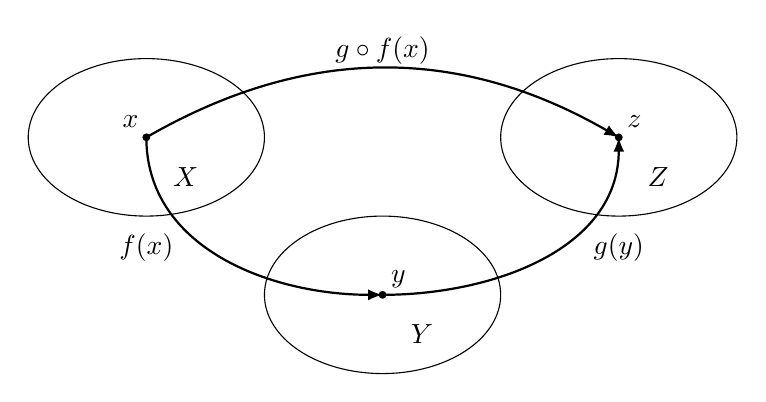
\begin{tikzpicture}[>= latex]
    \draw (-3 cm, 0) ellipse (1.5 cm and 1 cm);
    \draw ( 3 cm, 0) ellipse (1.5 cm and 1 cm);
    \draw ( 0   , -2 cm) ellipse (1.5 cm and 1 cm);

    \draw (-3, -1.4) node {$f(x)$};
    \draw[thick, ->] (-3, 0) to [out = -90, in = 180] (0, -2);

    \draw (3, -1.4) node {$g(y)$};
    \draw[thick, ->] (0, -2) to [out = 0, in = -90] (3, 0);

    \draw (0, 1.1) node {$g \circ f(x)$};
    \draw[thick, ->] (-3, 0) to [out = 30, in = 150] (3, 0);

    \fill (-3,0) circle (0.05);
    \draw (-3.2,.2) node {$x$};
    \draw (-2.5,-.5) node {$X$};

    \fill (0,-2) circle (0.05);
    \draw (0.2,-1.8) node {$y$};
    \draw (0.5,-2.5) node {$Y$};

    \fill (3,0) circle (.05);
    \draw (3.2,.2) node {$z$};
    \draw (3.5,-.5) node {$Z$};
  \end{tikzpicture}
  \caption{Композиция функций}
\end{figure}


}


\dfn{Сюръекция}{\textbf{Сюръективной функцией}
  называется $f: X \longrightarrow Y$, если
  $$\forall y \in Y \ \ \exists x \in X: y = f(x) \text{,}$$
  или иначе $Y = f(D)$.
}

\ex{}{
  $ \sin : \ \bbR \longrightarrow \bbR $ --- не сюръекция \\
  $ \sin : \ \bbR \longrightarrow [1;-1] $ --- сюръекция
}

\dfn{Инъекция}{\textbf{Инъективной функцией}
  называется $f: X \longrightarrow Y$, если
  $$\forall x_1, x_2 \in X: f(x_1) = f(x_2) \Rightarrow x_1 = x_2 \text{,}$$
 т. е. разным значениям аргумента соответсвуют разные значения функции. 
}

\dfn{Биекция}{\textbf{Биективной функцией (биекцией или взаимно-однозначным соответсвием)}
  называется сюръективная и инъективная функция.
}

\dfn{Обратная функция}{
  Если $f: X \longrightarrow Y$ --- биекция, то функция
  $$ f^{-1} = \{ (y,x): y = f(x)\}$$
  также является биективной и называется \textbf{обратной}.
}



\section{Мощность множеств}
\subsection{Эквивалентность множеств}

\dfn{Эквивалентные множества}{
  Множества $A$ и $B$ называются \textbf{эквивалентными или равносильными} $ A \sim B $, если существует биекция между этими множествами, т. е. каждому элементу из $A$ можно поставить в соответствие один и только один элемент из $B$ и наоборот.
}

Из свойств биективного отображения легко получаются следующие утверждения:
\begin{itemize}
  \item $A \sim A$
  \item $A \sim B \Leftrightarrow A \sim A$
  \item $(A \sim B) \wedge (B \sim C) \Rightarrow A \sim C$
\end{itemize}

\clm{Общая характеристика понятия мощности множества}{}{
  \textbf{Мощность множества} есть характеристика множества, обобщающая понятие количества элементов конечного множества.\\
  Мощность множества $A$ обозначают:
  $|A|, \ \text{card} (A)$.
}

\nt{Конечные множества равномощны т. и т. т., когда они содержат одинаковое количество элементов.}


\thm{Теорема Кантора-Бернулли}{
  $$\begin{cases}
     A_1 \subset A, \ B_1 \subset B \\ A_1 \sim B, \ B_1 \sim A
   \end{cases}
   \Rightarrow A \sim B$$
   \textit{Приводится без доказательства.}
}

\dfn{Счетные мнежства}{
  \textbf{Счетным множествлом} называется бесконечное множество, равномощное множеству $\bbN$.
  $$ |\bbN| = \aleph_0 \text{ --- алеф нуль} $$
}

\textbf{Свойства счетных множеств}
\begin{enumerate}[label=\bfseries\tiny\protect\circled{\small\arabic*}]
  \item $A \text{ --- бесконечное множество} \Rightarrow  \exists A_1 \subset A: \ |A_1| = \aleph_0$
  \item $|A| = \aleph_0 \Rightarrow \forall A_1 \subset A: \ (|A_1| = n) \vee (|A_1| = \aleph_0)$
  \item $A_1 \cap A_2 \cap ... \cap A_k = A \Rightarrow n_1 + n_2 + ... +  n_k = n, \ n_i = |A_i|, \ n = |A|$
  \item $n_1 + n_2 + ... \leq \aleph_0$
  \item $\aleph_0 + n = \aleph_0 - n = \aleph_0$
  \item $\aleph_0 + \aleph_0 + ... = \aleph_0$
  \item $\aleph_0 \cdot \aleph_0 = \aleph_0$
\end{enumerate}


\subsection{Мощность континуума}

\thm{Несчетность интервала $(0;1)$}{
    Множество чисел на интервале $(0;1)$ несчетно:
    $$|(0;1)| \neq \aleph_0$$
    \textbf{Доказательство:\\} 
  Любое число $\alpha_i \in (0;1)$ может быть представлено в виде бесконечной десятичной дроби: $\alpha_i = 0, \overline{a_1^{i} a_2^{i} a_3^{i} \ldots}$. Предположим от противного, что $(0;1)$ --- счетно, тогда $(0;1) = \{ \alpha_1, \alpha_2, \alpha_3, \dots\}$.
  Запишем числа $\alpha_i$ в столбец: 
  $$\begin{array}{lcl}
    \alpha_1 = 0, \overline{a_1^{1} a_2^{1} a_3^{1} \ldots}\\
    \alpha_2 = 0, \overline{a_1^{2} a_2^{2} a_3^{2} \ldots}\\
    \alpha_3 = 0, \overline{a_1^{3} a_2^{3} a_3^{3} \ldots}\\
    \ldots \ldots \ldots \ldots \ldots . \\
    \alpha_i = 0, \overline{a_1^{i} a_2^{i} a_3^{i} \ldots}\\
    \ldots \ldots \ldots \ldots \ldots . \\
  \end{array}$$
  Теперь посторим число $\beta =  0, \overline{b_1 b_2 b_3 \ldots}\  \in (0;1)$ следующим образом: за $b_1$ выберем любую цифру, отличную от $a_1^1$, за $b_2$ --- отличную от $a_2^2$, \ldots, за $b_i$ --- отличную от $a_i^i$, \ldots Таким образом, построено число из интервала $(0;1)$, которое не является не одним из чисел $\alpha_1, \alpha_2, \alpha_3 \ldots$ Полученное противоречие доказывает теорему.\\
  Описанный метод доказательства называется \textit{диагональным методом Кантора}.
}

\thm{Несчетность множества $\bbR$}{
  $$\forall a, b \in \bbR: \ (0;1) \sim (a;b) \sim (a;b] \sim [a;b] \sim (0; +\infty) \sim \bbR $$
  \textit{Теорема приводится без доказательства.}
}

\dfn{Мощность множества}{
  \textbf{Мощностью множества} называется класс множеств эквивалентных данному.\\
  Множества могут иметь следующие мощности:
  \begin{enumerate}
    \item $|\varnothing| = 0$ --- нулевой кардинал
    \item $|\{ a_1, a_2, \ldots, a_n \}| = n$ --- конечный ненулевой кардинал
    \item $|\bbN| = \aleph_0$ --- самый малый кардинал  
    \item $\aleph_1$ --- самый малый несчетный кардинал
    \item $|\bbR| = c$ --- континуум кардинал
  \end{enumerate}
}

\thm{Континуум-гипотеза}{
  $$\aleph_1 = c \Leftrightarrow \nexists T: \ |\bbN| < |T| < |\bbR|$$
}



\section{Множество действительных чисел}
\subsection{Аксиоматика множества действительных чисел}

\dfn{Бинарная операция}{
  На множестве $X$ задана \textbf{бинарная операция} $R$, если задана функция:
  $$R: X \times X \longrightarrow X \text{.}$$
}

\dfn{Множество действительных чисел}{
  \textbf{Множеством действительных чисел} называется любое множество $\bbR$, удовлетворяющее системе аксиом, называемых аксиомами множества действительных чисел:
  \begin{enumerate}[label = \Roman*.]
    \item \textbf{Аксиомы сложения:} на $\bbR$ задана бинарная операция $+: \bbR \times \bbR \longrightarrow \bbR$, называемая сложением, которая каждой паре элементов $x, y \in \bbR$ ставит в соответствие элемент $(x+y) \in \bbR$, называемый суммой элементов $x$ и $y$, и удовлетворяющая следующим условиям:
      \begin{enumerate}[label = \alph*.]
        \item $\forall x, y \in \bbR: \ x + y = y + x$ --- коммутативность сложения
        \item $\forall x, y, z \in \bbR: \ (x + y) + z = x + (y + z)$ --- ассоциативность сложения
        \item $\exists 0 \in \bbR \ \forall x \in \bbR: \ 0 + x = x + 0 = x$ --- существование нейтрального элемента относительно сложения
        \item $\forall x \in \bbR \ \exists (-x) \in \bbR: \ x + (-x) = 0$ --- существование противоположного элемента
      \end{enumerate}
    \item \textbf{Аксиомы умножения:} на $\bbR$ задана бинарная операция $\cdot: \bbR \times \bbR \longrightarrow \bbR$, называемая умножением, которая каждой паре элементов $x, y \in \bbR$ ставит в соответствие элемент $(xy) \in \bbR$, называемый произведением элементов $x$ и $y$, и удовлетворяющая следующим условиям:
      \begin{enumerate}[label = \alph*.]
        \item $\forall x, y \in \bbR: \ x \cdot y = y \cdot x$ --- коммутативность умножения 
        \item $\forall x, y, z \in \bbR: \ (x \cdot y) \cdot z = x \cdot (y \cdot z)$ --- ассоциативность умножения
        \item $\exists 1 \in \bbR \ \forall x \in \bbR: \ 1 \cdot x = x \cdot 1 = x$ --- существование нейтрального элемента относительно умножения 
        \item $\forall x \in \bbR \ \exists (x^{-1}) \in \bbR: \ x + x^{-1} = 0$ --- существование противоположного элемента
      \end{enumerate}
    \item \textbf{Связь операций сложения и умножения:}
      \begin{enumerate}[label = \alph*.]
        \item $\forall x, y, z \in \bbR: \ x \cdot (y + z) = x \cdot y + x \cdot y$ --- дистрибутивность
      \end{enumerate}
    \item \textbf{Аксиомы порядка:} на $\bbR$ задано отношение порядка $\leq$, удовлетворяющее условиям:
      \begin{enumerate}[label = \alph*.]
        \item $\forall x \in \bbR: \ x \leq x$ --- рефлексивность
        \item $\forall x, y \in \bbR: \ (x \leq y) \wedge (y \leq x) \Rightarrow x=y$
        \item $\forall x, y, z \in \bbR: \ (x \leq y) \wedge (y \leq z) \Rightarrow x \leq z$ --- транзитивность
        \item $\forall x, y\in \bbR: \ (x \leq y) \vee (y \leq x)$ 
      \end{enumerate}
    \item \textbf{Связь операций сложения, умножения и отношения порядка:}
      \begin{enumerate}[label = \alph*.]
        \item $\forall x, y, z \in \bbR: \ x \leq y \Rightarrow x + z \leq y + z$
        \item $\forall x, y, z \in \bbR, \ z > 0: \ x \leq y \Rightarrow x \cdot z \leq y \cdot z$
      \end{enumerate}
    \item \textbf{Аксиома полноты:}
      \begin{enumerate}[label = \alph*.]
        \item $\forall X, Y \subset \bbR, \ \forall x \in X, y \in Y: x \leq y \Rightarrow \forall x \in X, y \in Y \ \exists c \in \bbR: \ x \leq c \leq y$

      \end{enumerate}

  \end{enumerate}
}

\dfn{Модель множества $\bbR$}{
  \textbf{Моделью множества действительных чисел} называется любая конкретная реализация множества $\bbR$, удовлетворяющая перечисленным аксиомам.
}

\dfn{Изоморфизм}{
  \textbf{Изоморфизмом} называется биективное отображение $f: \bbR_1 \longrightarrow \bbR_2$, где $R_1$ и $R_2$ --- модели множества действительных числ, которое удовлетворяет следующим условиям:
  \begin{enumerate}
    \item $\forall x, y \in \bbR_1: \ f(x + y)= f(x) + f(y)$
    \item $\forall x, y \in \bbR_1: \ f(x \cdot y)= f(x) \cdot f(y)$
    \item $\forall x, y \in \bbR_1: \ x \leq y \Rightarrow f(x) \leq f(y)$
  \end{enumerate}
}



\subsection{Важнейшие подмножества}

\begin{enumerate}
  \item Множество натуральных чисел:
    $$ \bbN = \{ 1, 2, 3, \ldots \}$$
  \item Множество целых чисел:
    $$ \bbZ = \bbN \cup \{0\} \cup \{-1, -2, -3, \ldots \} $$
  \item Множество рациональных чисел:
    $$ \bbQ = \left\{ \frac{p}{q}: \ p \in \bbZ, \ q \in \bbN \right\}$$
  \item Промежутки $(a < b, \ a,b \in \bbR)$:
    \begin{enumerate}
      \item $[a, b] = \left\{ x \in \bbR: \ a \leq x \leq b \right\}$ --- отрезок
      \item $(a, b) = \left\{ x \in \bbR: \ a < x < b \right\}$ --- интервал 
      \item $[a, b) = \left\{ x \in \bbR: \ a \leq x < b \right\}$ --- полуинтервал 
      \item $(a, b] = \left\{ x \in \bbR: \ a < x \leq b \right\}$ --- полуинтервал 
      \item $\langle a, b \rangle = \left\{ [a,b], (a,b), [a,b), (a,b] \right\}$
    \end{enumerate}
\end{enumerate}



\subsection{Бесконечные десятичные дроби}

\dfn{Конечная десятичная дробь}{
  \textbf{Конечной десятичной дробью} называется десятичная дробь, имеющая конечное число знаков после запятой:
  $$ \overline{a,a_0a_1a_2a_3\ldots a_n}$$
}

\dfn{Бесконечная периодическая десятичная дробь}{
  \textbf{Бесконечной десятичной периодической дробью} называется десятичная дробь, имеющая бесконечное количество знаков после запятой, но начиная с некоторого знака, имеющая бесконечно повторяющуюся группу цифр (называемую \textbf{периодом}): 
  $$ \overline{a, a_0 a_1 a_2 \ldots a_n \underbrace{b_1 b_2 \ldots b_k}_{\text{период}} b_1 b_2 \ldots b_k \ldots b_1 b_2 \ldots b_k \ldots} $$
}

\nt{
  Любую конечную десятичную дробь можно считать бесконечной периодической дробью с нулем в периоде:
  $$2.5 = 2.500 \ldots 0 \ldots = 2.5(0)$$
}

\nt{
  Любое рациональное число может быть представлено в виде бесконечной периодической десятичной дроби.
}

\nt{
  Любая бесконечная десятичная периодическая дробь может быть представлена в виде обычной дроби при помощи представления первой в виде бесконечно убывающей геометрической прогрессии:
  $$1.(45) = 1 + \frac{45}{10^2} + \frac{45}{10^4} + \ldots = \left[ S = \frac{1}{1-q}, \ |q| < 1 \right] = 1 + \frac{1}{1 - \frac{1}{45}} = \frac{100}{55} = \frac{20}{11}$$
}

\nt{
  Бесконечные периодические дроби, имеющие 0 и 9 в периоде, представляются одной и той же обыкновенной дробью. Для определения взаимнооднозначного соответствия между обыкновенными и бесконечными дробями числа с 9 в периоде по договорённости не используются.
}

\dfn{Множество действительных чисел $\bbR$}{
  \textbf{Множеством действительных чисел} называется множество всех дробей вида:
  $$(1) \ \ \pm \overline{a_0,a_1 a_2 \ldots a_n \ldots}, \ a_0 > 0, \ a_k \in \{ 0, 1, \ldots, 9\}$$
}

\dfn{Множество иррациональных чисел}{
  \textbf{Множеством иррациональных чисел $\bbI$} называется множество всех дробей вида (1), которые не являются периодическими.
}

\dfn{Расширенная числовая прямая}{
  \textbf{Расширенной числовой прямой} называется дополнение множества $\bbR$ символами $+\infty$ и $-\infty$:
  $$\tilde{\bbR} = \{-\infty \} \cup \bbR \cup \{ +\infty \}$$
  Если дополнительно $\forall x \in \bbR: \ -\infty < x < +\infty$, то такое расширение называется \textbf{упорядоченным}.
}

\nt{
  \begin{itemize}
    \item $(+\infty) + (+\infty) = +\infty$
    \item $(-\infty) + (-\infty) = +\infty$
    \item $(+\infty) \cdot (+\infty) = (-\infty) \cdot (-\infty) = +\infty$
    \item $ \forall x > 0: \
      \begin{cases}
        x \cdot (+\infty) = +\infty \\
        x \cdot (-\infty) = -\infty \\
        x + (+\infty) = +\infty \\
        x - (+\infty) = -\infty \\
      \end{cases}
      , \ \forall x <0 : \
      \begin{cases}
        x \cdot (+\infty) = -\infty \\
        x \cdot (-\infty) = +\infty \\
        x + (+\infty) = +\infty \\
        x - (+\infty) = -\infty \\
      \end{cases}$
    \item $(+\infty) - (+\infty) = \text{неопределенность}$
    \item $\frac{\infty}{\infty} = \text{неопределенность}$
  \end{itemize}
}

\dfn{Упорядоченное расширение $\bbR$}{
  \textbf{Упорядоченным расширением $\bbR$} называется дополнением $\bbR$ символом $\infty$ (бесконечности):
  $$ \hat{\bbR} = \bbR \cup \{ \infty \} $$
}



\subsection{Границы числовых множеств}

\dfn{Максимальный элемент множества}{
  Пусть $\varnothing = X \subset \bbR$. \textbf{Максимальным элементом множества $X$} называется число $\max X  = M \in X$, для которого выполнено: $\forall x \in X: \ x \leq M$.
}

\dfn{Минимальный элемент множества}{
  Пусть $\varnothing = X \subset \bbR$. \textbf{Минимальным элементом множества $X$} называется число $\min X  = m \in X$, для которого выполнено: $\forall x \in X: \ m \leq x$.
}

\nt{
  У любого непустого конечного множества есть минимальный и максимальный элементы. Однако у бесконечного множества минимальный и максимальный элементы могут остутствовать.
}

\dfn{Верхняя граница множества}{
  \textbf{Верхней границей множества} $\varnothing \neq X \subset \bbR$ называется число $M \in \bbR$, для которого выполнено: $\forall x \in X: \ x \leq M$.
  \textit{\\ Верхняя граница не обязана принадлежать множеству!}
}

\nt{
  Если $M$ --- верхняя граница множества $X$, то $\forall M'>M$ тоже является верхней границей, т. е. верхних границ может быть бесконечно много.
}

\dfn{Ограниченность множества сверху}{
  Множество называется \textbf{ограниченным сверху}, если у него существует верхняя граница.
}

\dfn{Supremum a.k.a. точная верхняя граница}{
  Число $\sup X = M \in \bbR$ называется \textbf{супремумом или точной верхней границей} множества $\varnothing \neq X \subset \bbR$, если выполнены следующие условия:
  \begin{enumerate}
    \item $\forall x \in X: \ x \leq M$
    \item $\forall M' < M \ \exists x' \in X: \ M' < x' \leq M$
  \end{enumerate}
}

\nt{
  Первое условие определения постулирует, что точная верхняя граница сама является верхней границей. Второе условие утверждает, что при всяком уменьшении точной границы последняя перестанет быть точной верхней границей.
}

\dfn{Supremum в терминах $\epsilon$}{
   Число $\sup X = M \in \bbR$ называется \textbf{супремумом или точной верхней границей} множества $\varnothing \neq X \subset \bbR$, если выполнены следующие условия:
  \begin{enumerate}
    \item $\forall x \in X: \ x \leq M$
    \item $\forall \eps > 0 \ \exists x' \in X: \ M - \eps < x' \leq M$
  \end{enumerate}
}

\nt{
  Супремум --- наименьшая из верхних границ множества. Супремум может как принадлежать, так и не принадлежать множеству.
}

\dfn{Нижняя граница множества}{
  \textbf{Нижней границей множества} $\varnothing \neq X \subset \bbR$ называется число $m \in \bbR$, для которого выполнено: $\forall x \in X: \ m \leq x$.
}

\dfn{Ограниченность множества снизу}{
  Множество называется \textbf{ограниченным снизу}, если у него существует нижняя граница.
}

\dfn{Infimum a.k.a. точная нижняя граница}{
  Число $\inf X = m \in \bbR$ называется \textbf{инфимумом или точной нижней границей} множества $\varnothing \neq X \subset \bbR$, если выполнены следующие условия:
  \begin{enumerate}
    \item $\forall x \in X: \ m \leq x$
    \item $\forall m' > m \ \exists x' \in X: \ m \leq x' < m'$
  \end{enumerate}
}

\dfn{Infimum a.k.a. точная нижняя граница}{
  Число $\inf X = m \in \bbR$ называется \textbf{инфимумом или точной нижней границей} множества $\varnothing \neq X \subset \bbR$, если выполнены следующие условия:
  \begin{enumerate}
    \item $\forall x \in X: \ m \leq x$
    \item $\forall \eps > 0 \ \exists x' \in X: \ m \leq x' < m + \eps$
  \end{enumerate}
}

\nt{
  Если множество $\varnothing \neq X \subset \bbR$ не является ограниченным сверху (снизу), то полагают:
  $$\sup X = +\infty \ \ (\inf X = -\infty)$$
}

\dfn{Ограниченное множество}{
  Множесвтво $\varnothing \neq X \subset \bbR$ называется \textbf{ограниченным}, если оно ограничено сверху и снизу, иначе:
  $$ X \text{ --- ограничено } \xLeftrightarrow{\text{def}} \ \exists m, M \in \bbR \ \forall x \in X: \ m \leq x \leq M$$
}

\pagebreak
\clm{}{}{
  \begin{itemize}
    \item $\sup X$ и $\inf X$ определяются однозначно
    \item $\exists \max X \Rightarrow \max X = \sup X$
    \item $\exists \min X \Rightarrow \min X = \inf X$
  \end{itemize}
}

\thm{Теорема Дедекинда}{
  \begin{enumerate}[label = \Roman*.]
    \item $
      \begin{cases}
        \varnothing \neq X \subset \bbR \\
        X \text{ --- ограничено сверху} \\
      \end{cases}
      \Rightarrow \exists \sup X$
     \item $
      \begin{cases}
        \varnothing \neq X \subset \bbR \\
        X \text{ --- ограничено снизу} \\
      \end{cases}
      \Rightarrow \exists \inf X$
  \end{enumerate}

  \textbf{Доказательство: \\}
  Докажем первое утверждение. Пусть $Y$ --- множество верхних границ $X$. В силу ограниченности $X$ множество $Y$ непусто.
  $$ \forall x \in X \ \forall y \in Y: \ x \leq y \xRightarrow{\text{аксиома полноты}} \exists M \in \bbR \ \forall x \in X  \ \forall y \in Y: \ x \leq M \leq y$$
  $$ x \leq M \ \forall x \in X \Rightarrow M \text{ --- верхняя граница } X \Rightarrow M \in Y$$
  $$ (\forall y \in Y: \ M \leq y) \wedge (M \in Y) \xRightarrow{def} M = \min Y \Rightarrow M = \sup X$$
}



\subsection{Принцип Архимеда}

\mlenma{Cуществование минимума ограниченного подмножества целых чисел}{
  \[
    \varnothing \neq A \subset \bbZ \text{ --- ограничено сверху (снизу)} \Rightarrow \exists \max A \ (\min A)
  .\] 
  \textbf{Доказательство:} \\
  Докажем лемму для случая ограниченного сверху множества.
  $$ A \text{ --- огр. сверху} \xRightarrow{\text{т. Дедекинда}} \exists \sup A = M \xRightarrow{\text{def sup}} \exists n \in A: \ M - 1 < n \leq M \Rightarrow$$
  $$\Rightarrow M < n+1 \Rightarrow n+1 \notin A \Rightarrow \forall k \in \bbN: \ n+k \notin A \Rightarrow n = \max A$$
}

\mlenma{Принцип Архимеда}{
  $$ \forall x \in \bbR \ \ \forall h>0 \ \ \exists! n \in \bbZ: \ nh \leq x < (n+1)h$$
  \textbf{Доказательство:}\\
  Рассмотрим множество $A = \{ k \in \bbZ: \ k \leq \frac{x}{h} \}$.
  $$ A \text{ --- огр. сверху} \xRightarrow{\text{Лемма 1.6.1}} \exists \max A = n \Rightarrow n \leq \frac{x}{h} < n+1 \Rightarrow nh \leq x < (n + 1)h$$
}

\cor{}{
  $$\forall x \in \bbR \ \ \exists! n \in \bbZ: \ n \leq x < n + 1$$
}

\dfn{Целая и дробная часть числа}{
  \textbf{Целой частью числа} $[x]$ называется число, не превышающее заданное число $x$.
  $$[x], \ [5.2] = 5, \ [-3.2] = -4$$
  \textbf{Дробной частью числа} называется число $\{x\} = x - [x]$.
}

\thm{Плотность $\bbQ$ в $\bbR$}{
  $$\forall a, b \in \bbR, \ a<b: \ (a;b) \cap \bbQ \neq \varnothing$$
  \textbf{Доказательство:}\\
  Путь $h_1 = b - a$. Согласно принципу Архимеда, $\exists n \in \bbN: 1 < nh_1 \Rightarrow  \frac{1}{n} < h_1$. Применим принцип Архимеда к числу $a$ с $h = \frac{1}{n}$:
  $$\exists m \in \bbZ: \ \frac{m}{n} \leq a < \frac{m+1}{n} = \frac{m}{n} + \frac{1}{n} < \frac{m}{n} + h_1 \leq a + b - a = b$$
  $$\Downarrow$$
  $$r = \frac{m+1}{n} \in (a;b), \ r \in \bbQ$$
}
